\documentclass{article}
\usepackage[hidelinks]{hyperref}
\usepackage{graphicx}
\usepackage{amsfonts}
\usepackage{amsmath}
\usepackage{enumitem}
\usepackage{polski}
\usepackage[utf8]{inputenc}
\usepackage{indentfirst}
\usepackage{float}
\title{Dokumentacja projektu dotyczącego optymalnego układania klocków na planszy}
\author{Abdelkarim Ahmed, Cacko Agata, Hernik Aleksandra}
\begin{document}
\maketitle
\section{Opis projektu}
Tematem naszego projektu jest stworzenie aplikacji przedstawiającej algorytm układania klocków na planszy (nazywanej również studnią) tak, aby ich wysokość była jak najmniejsza. Klocki nie mogą się nakładać, a szerokość studni określana jest z góry. Wykorzystanym algorytmem jest algorytm zachłanny z nawrotami.



\begin{figure}[H]
\begin{center}
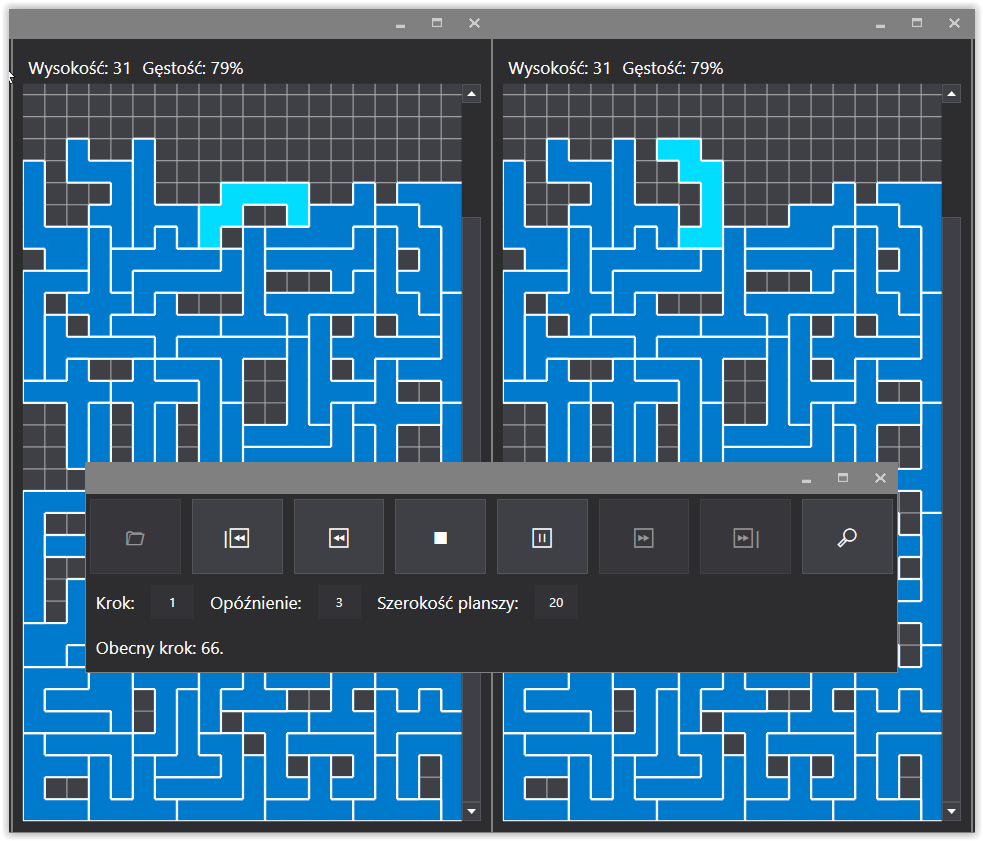
\includegraphics[width=0.9\textwidth]{interfejs.png}
\end{center}
\vspace{-0.3cm}
\caption{Wygląd interfejsu wraz z przykładowym wywołaniem}
\end{figure}



\subsection{Zewnętrzne biblioteki}

W celu stworzenia wygodnego interfejsu posłużyliśmy się następującymi bibliotekami zewnętrznymi:


\begin{itemize}
\item \textbf{MicroMVVM} -- biblioteka ułatwiająca pisanie aplikacji zgodnie ze wzorcem projektowym MVVM, strona projektu: \\ \url{https://micromvvm.codeplex.com/}
\item \textbf{Visual Studio 2012 Metro Styles for WPF} -- biblioteka zapewniająca ładny wygląd interfejsu, strona projektu: \url{https://www.codeproject.com/articles/442856/visual-studio-metro-styles-for-wpf}
\end{itemize}




%\clearpage
\section{Opis algorytmu}
Wykorzystany algorytm jest algorytmem zachłannym z określoną parametrem liczbą nawrotów $k$. W każdym kroku algorytmu uruchamiane jest $k'$, gdzie $1 \le k' \le k$ (w sekcji wielowątkowość znajduje się wyjaśnienie, od czego jest uzależniona ich dokładna liczba). Każdemu wątkowi odpowiada jeden z $k$ najlepszych wyników uzyskanych w poprzednim kroku, gdzie najlepszy wynik to taki, dla którego wartość funkcji kosztu jest jak najmniejsza -- każdy z nich dla swoich danych wejściowych znajduje $k$ najlepszych rozwiązań. Znalezienie rozwiązań polega na sprawdzeniu dla każdego klocka każdego jego rotacji -- najpierw wybierana jest jego pozycja, a następnie liczony koszt całej planszy. $k$ rozwiązań takich, że funkcja kosztu obliczona na planszy z położonym danym klockiem w danej rotacji jest najmniejsza, to rozwiązanie dla danego wątku. Następnie, spośród ułożeń otrzymanych przez wszystkie wątki ($1 \le k' \le k$, zatem otrzymywane jest od $k$ do $k^2$ ułożeń) wybierane jest $k$ najlepszych. Ogólny schemat działania algorytmu podsumowuje poniższy diagram:
%\vspace{-0.3cm}
\begin{figure}[H]
\begin{center}
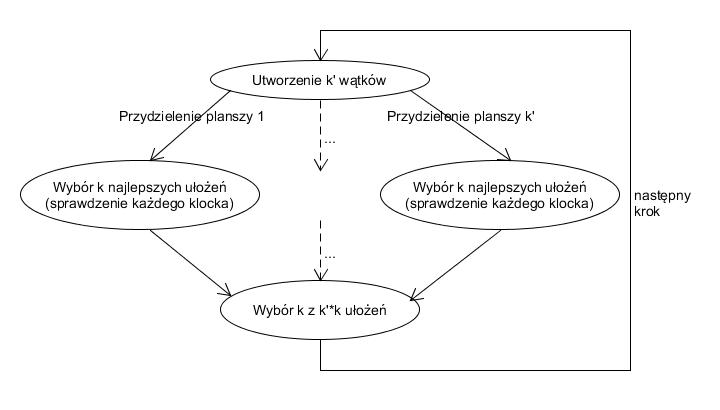
\includegraphics[width=0.85\textwidth]{schemat_algorytmu.png}
\end{center}
\caption{Ogólny schemat działania algorytmu}
\end{figure}

\subsection{Wybór pozycji dla klocka}
Funkcja wyboru pozycji klocka to \textit{PlacementFunction}. Zaimplementowaliśmy jedną taką funkcję -- dla każdego klocka wraz z numerem wersji (konkretnym obrotem) wybiera pierwsze wolne miejsce. Sprawdzane są kolejne pozycje (wierszami od dołu, a następnie od lewej). Wolne miejsce oznacza, że można położyć klocek o danym obrocie w taki sposób, że każde pole zajęte przez niego było wcześniej puste.

Testowaliśmy również funkcję, która zamiast zwracać jedną możliwą pozycję klocka, zwracała wszystkie możliwości. Wbrew intuicji wyniki algorytmu z jej zastosowaniem były gorsze, a ponadto nastąpił znaczny spadek wydajności, dlatego ostatecznie ją odrzuciliśmy.



\subsection{Funkcje kosztu planszy}
Aplikacja umożliwia wybór funkcji kosztu, która jest wykorzystywana w trakcie działania algorytmu. Wszystkie funkcje kosztu przyjmują jako parametr planszę i zwracają liczbę całkowitą -- im niższy wynik, tym lepsze rozwiązanie. Dostępne są następujące funkcje:
\begin{itemize}
\item \textit{Najmniej dziur} -- wynik to liczba dziur, przy czym dziura jest definiowana jako każde puste pole takie, że co najmniej jedno pole znajdujące się wyżej jest zajęte.
\item \textit{Najmniejsza wysokość} -- wynik to wysokość najwyższej kolumny.
\item \textit{Największa przyległość} -- wynik to wartość przeciwna do sumy długości fragmentów krawędzi klocków, które przylegają do innych klocków lub ścian.
\item \textit{Najładniejsze puste pola} -- funkcja eksperymentalna, której wynik to iloraz liczby dziur, definiowanych tak jak w funkcji \textit{Najmniej dziur}, i liczby zapełnionych pól.
\item \textit{Najmniej dziur ze średnią} -- wprowadzona pod koniec testów usprawniona wersja funkcji minimalizującej liczbę dziur. Usprawnienie polega na tym, że jako dziury liczone są również puste pola znajdujące się poniżej zaokrąglonej średniej z wysokości kolumn, co zapobiega tworzeniu ``kominów''.
\end{itemize}
\subsection{Wielowątkowość}
W celu przyspieszenia działania algorytmu, do wykonywania niezależnych od siebie obliczeń wykorzystywany jest mechanizm wątków. W tym przypadku takimi obliczeniami jest szukanie $k$ najlepszych rozwiązań dla danej planszy. W każdym kroku tworzone jest $k'$ wątków, gdzie $1 \le k' \le k$, a w większości przypadków $k'=k$. 

Pierwszym ze szczególnych przypadków jest pierwszy krok - ponieważ jest tylko jedno wcześniejsze ułożenie (pusta plansza), uruchamiany jest tylko jeden wątek -- gdyby było uruchomione k wątków, każdy z nich znalazł by te same rozwiązania i w efekcie algorytm wybrałby najlepsze rozwiązanie z każdego wątku -- czyli wynikiem pierwszego kroku byłoby k identycznych ułożeń. Dzięki uruchomieniu tylko jednego wątku, znajdowane jest k różnych ułożeń, a ponadto, szczególnie dla dużych k, wykonuje się on szybciej. 

Drugi przypadek jest efektem dodatkowego usprawnienia algorytmu, który ma na celu eliminowanie identycznych rozwiązań, w celu sprawdzenia jak największej liczby możliwości. Polega ono na tym, że po każdym kroku sprawdzana jest unikalność rozwiązań -- sprawdzany jest najpierw ostatni położony klocek (współrzędne, w których został położony, obrót i identyfikator). Jeśli wykryty zostanie jakikolwiek konflikt, dokonywane jest porównanie plansz wynikowych. W przypadku, gdy plansze również są identyczne, pozostawiane jest tylko jedno z tych rozwiązań -- bo identyczne plansze dają identyczne rozwiązania, więc dopóki jakieś rozwiązanie pochodzące z tej planszy byłoby jednym z $k$ najlepszych istniejących, dwa wątki wykonywałyby dokładnie te same operacje. W ten sposób do następnego kroku może trafić zredukowana liczba plansz wejściowych, ale krok później, o ile znowu nie występowały powtórzenia, algorytm stabilizuje liczbę wątków na $k$. Koszt takiego rozwiązania jest niewielki -- porównanie wstępne jest realizowane w czasie stałym (liczba porównań jest rzędu $k^2$, gdzie $k$ to stała, a porównanie ułożenia klocka to cztery porównania liczb całkowitych), więc jeśli problem nie wystąpi, algorytm nie działa zauważalnie wolniej. Liczba sytuacji, w których trzeba wykonać dodatkowe sprawdzenie, powinna być bardzo niewielka, a eliminacja identycznych rozwiązań eliminuje jednakowe obliczenia, które mogłyby ciągnąć się nawet do samego końca -- efektywnie algorytm działałby od pewnego momentu tak, jakby wartość $k$ została zmniejszona.

Po zwróceniu przez każdy z $k$ wątków listy $k$ najlepszych rozwiązań trzeba wybrać k najlepszych rozwiązań z otrzymanych $k^2$.  
Wynikowe elementy są wybierane przez k-krotny wybór największego elementu z list.
Korzystamy tu z faktu, że zwrócone listy są posortowane po wartości funkcji kosztu.
Dzięki temu wystarczy sprawdzić tylko najmniejszy niewykorzystany element z każdej listy (w czasie $k$), zamiast przeglądać wszystkie elementy wszystkich list (w~czasie~$k^2$).
\subsection{Struktura danych}


\subsubsection{Klasy klocków}
\begin{itemize}
\item \textbf{BlockType} -- najbardziej podstawowa klasa. Zawiera informację o kształcie klocka (tablica intów, 0 oznacza pole wolne, 1 pole zajęte przez klocek) oraz jego \textit{Id} (unikalne dla typu klocka). W celu ułatwienia implementacji algorytmu i optymalizacji czasowej przy tworzeniu instancji klasy tworzone są też wszystkie rotacje, a potem usuwane duplikaty. Co więcej pierwsza wersja klocka, tj. tablica na samym początku listy \textit{Shape}, jest zawsze pozioma -- tj. jej szerokość jest większa lub równa wysokości. Każda kolejna wersja jest obrócona względem poprzedniej o kąt prosty.
\item \textbf{BlockInstance} -- struktura reprezentująca jeden konkretny klocek ułożony na planszy. Zawiera obiekt klasy \textit{BlockType}, współrzędne położenia oraz numer wersji klocka (numer obrotu, czyli indeks na liście \textit{Shape} w obiekcie \textit{BlockType}). Dodatkowo znajduje się tu również wskaźnik na poprzedni dodany klocek (por. \ref{ref:stepsdata}).
\item \textbf{PartialSolution} -- klasa zawierająca obiekt \textit{BlockInstance} i wartość funkcji kosztu, zastosowanej do pewnej planszy, na której został ułożony dany klocek. Lista obiektów tej klasy zwracana jest przez funkcję \textit{ChooseBlocks}.
\end{itemize}


\subsubsection{Klasa Algorithm}
Główną klasą naszego programu jest klasa Algorithm. Przechowuje ona wszystkie dane dotyczące algorytmu i wykonuje kolejne kroki. Zawiera tablicę obiektów klasy \textit{Board}, przechowującą stany wszystkich plansz w danym kroku algorytmu, oraz StepsData, przechowujące dane o przebiegu algorytmu. Ponadto w klasie \textit{Algorithm} znajduje się funkcja łączenia wyników (wybierania $k$ najlepszych z $k^2$ możliwych ułożeń).

Klasa zawiera również funkcję kosztu i funkcję wyboru miejsca na klocek, oraz słownik dostępnych klocków (dane powtórzone z klasy \textit{Data}, jednak to powtórzenie jest przydatne -- przy tworzeniu nowych obiektów \textit{Board} potrzebny jest nowy słownik dostępności klocków, a dużo szybciej i przy mniejszej ilości kodu tworzy się go z innego słownika niż listy klocków).



\subsubsection{Klasa Board}
Klasa Board odpowiada za przechowywanie zawartości studni (jest to tablica intów). Przechowuje także słownik dostępności klocków (kluczami są typy klocków, wartościami -- liczba dostępnych klocków danego typu). Ponieważ operacje na słownikach są czasochłonne, przy tworzeniu klasy dajemy informację, czy chcemy, aby obiekt ,,śledził'' klocki -- tj. sprawdzał ich dostępność, dodawał i odejmował jeden do liczby dostępnych przy dodawaniu klocków i usuwaniu ich z planszy itd., czy nie. W przypadku plansz tymczasowych (wykorzystywanych w funkcji \textit{ChooseBlocks}) oraz przy tworzeniu widoku śledzenie dostępności klocków nie jest potrzebne, ponieważ mamy pewność, że dodajemy właściwe klocki.



Ważne metody:
\begin{itemize}
\item \textbf{AddBlock} -- sprawdza możliwość dodania klocka na planszę (czy miejsce, w które chcemy położyć klocek, jest wolne, oraz czy w ogóle mamy dostępny taki klocek), po czym zmniejsza o jeden liczbę dostępnych klocków tego typu i wpisuje klocek w odpowiednie miejsce na planszy.
\item \textbf{DeleteBlock} -- usuwa klocek ze studni. Nie ma żadnych mechanizmów weryfikacji, czy faktycznie klocek leżący w danym miejscu na planszy jest tym samym klockiem co ten, którego chcemy z planszy usunąć. Taka weryfikacja jednak nie jest potrzebna, ponieważ stosujemy algorytm zachłanny, zatem usuwanie klocków wcześniej położonych nie jest w ogóle potrzebne. W przypadku naszego programu stosowane jest to jednak przy wyborze najlepszego miejsca na kolejny klocek, gdy dodajemy i usuwamy kolejne klocki w różnych miejscach na tymczasowej planszy.
\item \textbf{ChooseBlocks} -- wybiera $k$ najlepszych ułożeń, gdzie ,,ułożenie'' to trójka: typ klocka, obrót i współrzędne miejsca, w które wkładamy klocek (współrzędne lewego dolnego rogu). Wszystkie te informacje znajdują się w obiektach klasy \textit{PartialSolution}. $k$ jest przekazywane jako parametr i może być dowolne, jednak w naszym programie zawsze jest to liczba rozgałęzień algorytmu.
\end{itemize}

\subsubsection{Klasa StepsData}
\label{ref:stepsdata}
Klasa ta zawiera zminimalizowane informacje o przebiegu algorytmu. Dzięki niej możemy łatwo odzwierciedlić stan algorytmu w danym kroku bez wykonywania dodatkowych obliczeń czy uruchamiania algorytmu ponownie.

Główną częścią klasy jest tablica struktur BlockInstance. Wiersze odpowiadają kolejnym krokom algorytmu, kolumny -- kolejnym studniom. Liczba wierszy jest równa liczbie klocków, a liczba kolumn -- liczbie rozgałęzień algorytmu.

W pierwszym kroku algorytmu wypełniany jest pierwszy wiersz tablicy. Każde kolejne pole to pierwszy klocek na danej planszy.

W kolejnym kroku algorytmu wypełniany jest kolejny wiersz tablicy. Ze wszystkich możliwości algorytm wybrał $k$ najlepszych ułożeń klocków na różnych planszach. Nie ma jednak pewności, że chcemy dołożyć klocek na każdą planszę z poprzednich $k$ plansz. Przeciwnie, kilka z tych $k$ najlepszych ułożeń może dotyczyć tej samej (poprzednio) planszy, a z kolei inna plansza zostanie całkowicie odrzucona. Rozwiązaniem tego problemu jest zapisanie $k$ ułożeń w kolejnym wierszu, oraz zapisanie tam informacji, jak odtworzyć planszę, na której chcemy położyć ten klocek. Wystarczy zapamiętać ,,wskaźnik'' do poprzedniego klocka. W tym przypadku -- numer kolumny, w której będziemy szukać poprzedniego klocka. Oczywiście poprzedni klocek dodaliśmy w poprzednim wierszu, więc numer wiersza jest znany.

W ten sposób powstaje pewna struktura drzewiasta, mająca na każdym poziomie dokładnie $k$ węzłów. Odtworzenie $i$-tego kroku algorytmu na $j$-tej planszy polega na dodawaniu kolejno klocka z $(i, j)$-tego elementu tablicy, klocka z $(i-1, BlockInstances[i, j].PreviousBlockBoardNumber)$-tego elementu tablicy itd. (\textit{BlockInstances} -- tablica struktur \textit{BlockInstance}, \textit{PreviousBlockBoardNumber} -- numer kolumny (numer planszy), w której znajduje się poprzedni klocek).

W celu ułatwienia korzystania z klasy, StepsData implementuje interfejs IEnumerable. Jest to jednak niestandardowy sposób implementacji. Przed użyciem polecenia \textit{foreach} należało użyć funkcji \textit{SetStartingPoint}, która ustawia współrzędne węzła, od którego zaczynamy przechodzić po drzewie. Kolejne węzły wybierane są w sposób opisany wyżej (jak przy odtwarzaniu planszy). Przy większym projekcie byłoby to złą praktyką, jednak przy tak małym ryzyko jest dużo mniejsze i wygoda tego rozwiązania przeważa.
%zastosowanie to nie jest obarczone dużym ryzykiem, 



\clearpage
\section{Wydajność}
Testy wydajnościowe były wykonywane na komputerze z dość starym procesorem AMD Phenom II X4 965 BE, który jest znacznie wolniejszy od procesora Intel Core i7 2600K w komputerach laboratoryjnych, a ponadto nie posiada funkcjonalności hyperthreading, która znacząco zwiększa wydajność aplikacji wielowątkowych. Mimo tego, wykonanie algorytmu nawet dla dużych zestawów danych trwało co najwyżej kilkadziesiąt sekund.

Pierwszy przeprowadzony test polegał na porównaniu wydajności funkcji kosztu dla zestawu 200, 400 i 600 klocków dla parametru $k = 4$. Rezultaty znajdują się na wykresie poniżej:
\begin{figure}[H]
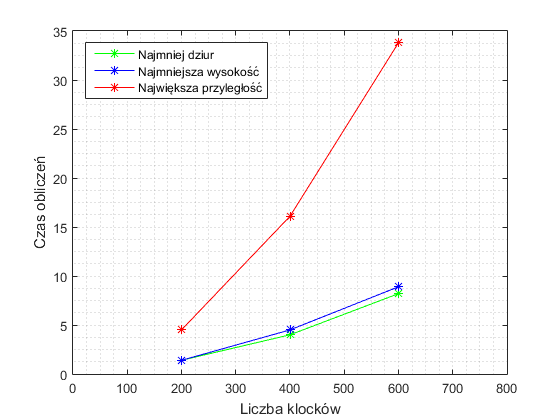
\includegraphics[width=\textwidth]{wydajnosc_porownanie_funkcji.png}
\caption{Porównanie wydajności funkcji kosztu}
\end{figure}
Jak widać, funkcja maksymalizująca przyległość jest znacznie wolniejsza od dwóch pozostałych, których wydajność jest prawie identyczna. Był to spodziewany rezultat, ponieważ ta funkcja dla każdego pola w tablicy musi dokonać pięciu sprawdzeń (czy fragment klocka dotyka lewej ściany, prawej ściany, podłogi, fragmentu innego klocka z prawej strony i fragmentu innego klocka na górze), w przeciwieństwie do pozostałych funkcji, które dokonują tylko jednego sprawdzenia. Spodziewanym rezultatem był również duży wpływ funkcji kosztu na czas działania całego algorytmu -- funkcja kosztu jest wywoływana w każdym kroku przez każdy wątek tyle razy, ile jest możliwych do uzyskania przez ten algorytm ułożeń.

Drugi test sprawdza wpływ zmiany parametru $k$ na wydajność algorytmu. Sprawdzane były wartości 1, 2, 3, 4, 6, 8 i 10 dla funkcji \textit{Najmniej dziur} oraz zestawu 200, 400 i 600 klocków. Poniższy wykres obrazuje wyniki:
\begin{figure}[H]
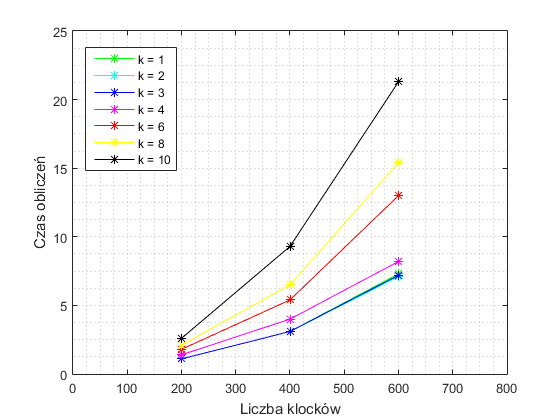
\includegraphics[width=\textwidth]{porownanie_k.png}
\caption{Porównanie wydajności dla różnych wartości parametru}
\end{figure}
Również w tym teście wyniki nie zaskakują. Wyniki dla wartości $k$ równych 1, 2 i 3 są identyczne, ponieważ procesor, na którym wykonywane były testy, ma cztery rdzenie -- jeden z nich zawsze jest częściowo wykorzystywany przez inne działające aplikacje (w tym system operacyjny), a także interfejs użytkownika. Pozostałe trzy w całości mogły poświęcić się liczeniu algorytmu. Stąd też bardzo niewielki skok przy zmianie $k$ z 3 na 4. Dalszy wzrost wynika przede wszystkim z braku możliwości rzeczywistego jednoczesnego obliczania wszystkich wątków i częściowo z narzutu wynikającego z ich tworzenia.

Zauważonym problemem jest znaczne spowolnienie działania interfejsu przy dużej liczbie klocków -- wynika to z ręcznego rysowania każdego fragmentu krawędzi klocka oddzielnie, co przypuszczalnie sprawia, że do karty graficznej przesyłane jest dużo małych poleceń rysowania, zamiast jednego większego. Dzięki temu jednak wizualizacja jest znacznie czytelniejsza niż w przypadku aplikacji, w których klocki oddzielane są jedynie kolorem. 
\clearpage



\section{Testy}
\subsection{Zestaw 100 klocków 4x3, 5x3, 5x4, 6x4 o polu co najwyżej 8}
Na tym standardowym zestawie klocków zostanie dokonana dokładna analiza własności naszego algorytmu z uwzględnieniem różnej liczby rozgałęzień, szerokości studni i wszystkich udostępnionych funkcji kosztu.

\subsubsection{Szerokość studni: 5}
\begin{enumerate}
\item Funkcja minimalizująca dziury

Gęstość dla $k=3$: 71

Najlepsza gęstość dla $k=5$: 71

Dla podanych parametrów można zauważyć ciekawe zachowanie. 
Wbrew oczekiwaniom zwiększaniu liczby rozgałęzień nie towarzyszy poprawa wyników. 
Najlepszy wynik wystąpił dla $k=5$ i $k=10$ przy znacznie niższych wartościach dla wartości pomiędzy. W
ynika to ze specyfiki zastosowanego algorytmu, będącego algorytmem zachłannym. 
Na przykład dla $k=4$ w trakcie obliczeń mogło pojawić się ułożenie, które w danym momencie wydawało się bardziej obiecujące, niż wszystkie ułożenia dla $k=3$, jednak ostatecznie okazało się mniej korzystne.
Podobny efekt można zaobserwować dla pozostałych funkcji.

\begin{figure}[H]
\centering
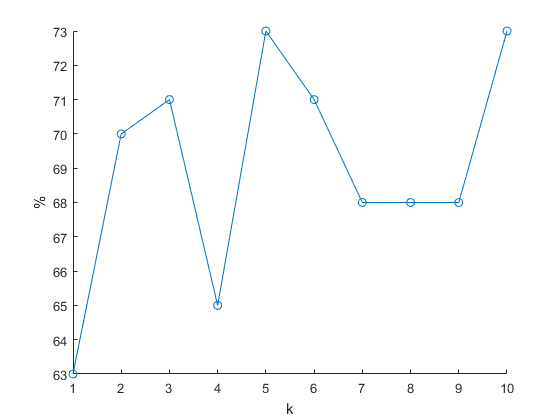
\includegraphics[width=0.90\textwidth]{k_plot.png}
\caption{Wykres gęstości od liczby rozgałęzień}
\end{figure}

\item Funkcja minimalizująca wysokość

Gęstość dla $k=3$: 71

Najlepsza gęstość dla $k=10$: 75

Funkcja wysokości, nie najlepiej sprawdzająca się w większości przypadków, przy wąskiej studni radzi sobie porównywalnie z pozostałymi.

\item Funkcja maksymalizująca przyleganie

Gęstość dla $k=3$: 70

Najlepsza gęstość dla $k=7$: 76

Jest to najlepsza funkcja dla tego przypadku - dobry rezultat udało się osiągnąć przy stosunkowo małej wartości k.
\end{enumerate}
\subsubsection{Szerokość studni: 20}
Szerokość 20 jest najlepsza do porównania funkcji kosztu, a także zaobserwowania ich szczególnych cech.
Pozwala na większą swobodę ułożenia klocków niż szerokość 5, a jednocześnie wynikowa wysokość jest na tyle duża, że nierówności na górze nie mają istotnego wpływu na gęstość.
\begin{enumerate}
\item Funkcja minimalizująca dziury

Gęstość dla $k=3$: 75

Najlepsza gęstość dla $k=9$: 80

Na rysunku można zaobserwować pewną wadę tej funkcji - pozwala na tworzenie głębokich, wąskich dziur (jak na górze po lewej). 
Wynika to z tego, że takie zjawisko nie jest traktowane przez funkcję jako dziura.
Z kolei zakrycie takiej dziury klockiem znacząco zwiększa liczbę dziur, więc algorytm pozwoli na to tylko w ostateczności.

\begin{figure}[H]
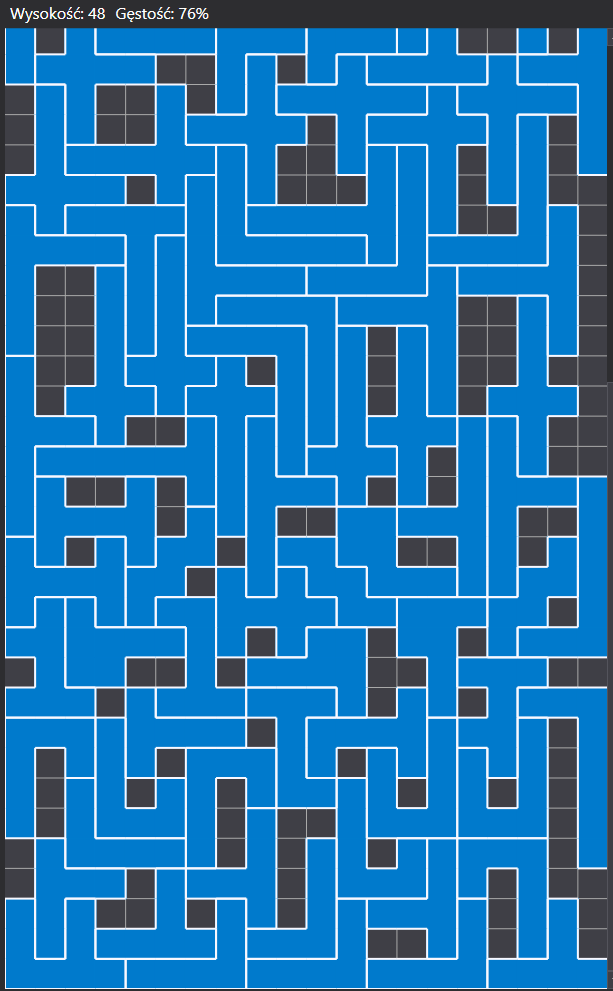
\includegraphics[width=\textwidth]{dziury.PNG}
\caption{Ułożenie klocków dla funkcji dziur}
\end{figure}

\item Funkcja minimalizująca wysokość

Gęstość dla $k=3$: 72

Najlepsza gęstość dla $k=10$: 76

W przypadku funkcji wysokości można zauważyć ciekawy wizualny efekt - klocki wydają się być położone maksymalnie poziomo.
Wynika to z faktu, że takie położenie minimalizuje wysokość w danym ruchu - nie ma znaczenia, że za kilka ruchów może się okazać niekorzystne.

\begin{figure}[H]
\centering
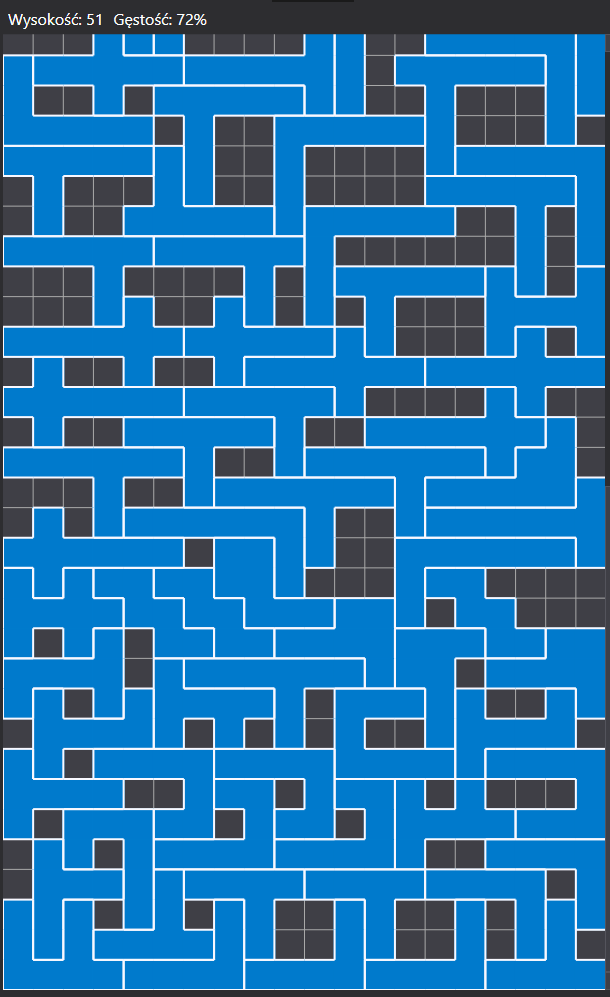
\includegraphics[width=0.72\textwidth]{wysokosc.PNG}
\caption{Ułożenie klocków dla funkcji wysokości}
\end{figure}

\item Funkcja maksymalizująca przyleganie

Gęstość dla $k=3$: 76

Najlepsza gęstość dla $k=8$: 83

Funkcja przylegania sprawdziła się w tym przypadku najlepiej.

\begin{figure}[H]
\centering
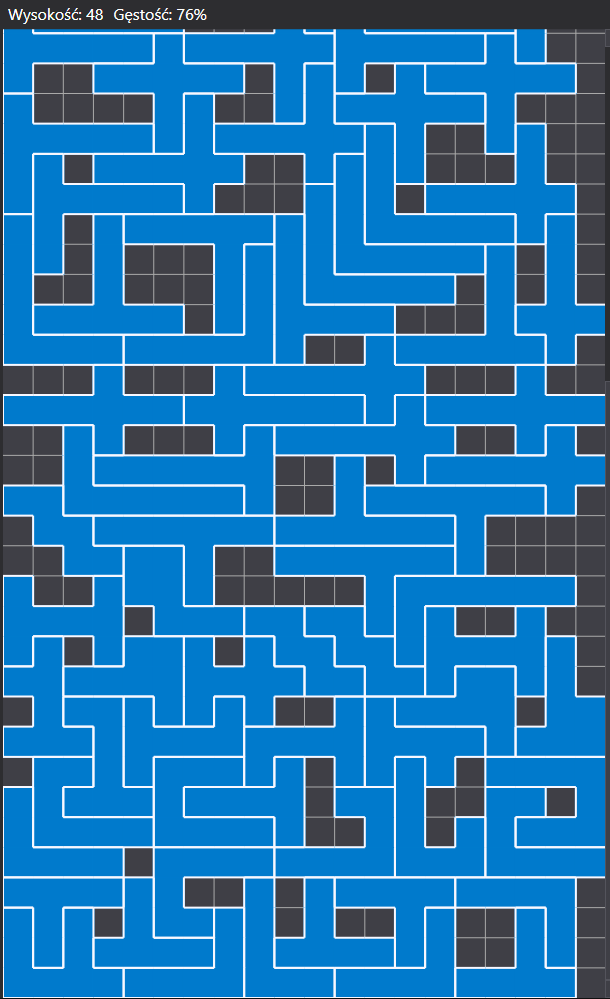
\includegraphics[width=0.8\textwidth]{przyleglosc.PNG}
\caption{Ułożenie klocków dla funkcji przyległości}
\end{figure}

\end{enumerate}
\subsubsection{Szerokość studni: 80}
\begin{enumerate}

\item Funkcja minimalizująca dziury

Gęstość dla $k=3$: 66

Najlepsza gęstość dla $k=5$: 71

\begin{figure}[H]
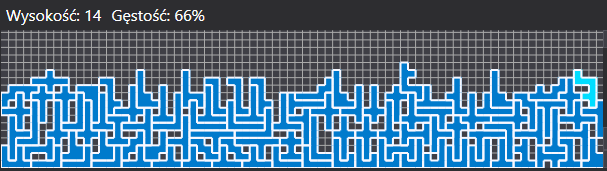
\includegraphics[width=\textwidth]{szeroka_plansza.PNG}
\caption{Ułożenie klocków dla funkcji przyległości}
\end{figure}

\item Funkcja minimalizująca wysokość

Gęstość dla $k=3$: 66

Najlepsza gęstość dla $k=9$: 66

\item Funkcja maksymalizująca przyleganie

Gęstość dla $k=3$: 66

Najlepsza gęstość dla $k=5$: 71

\end{enumerate}
\textbf{Wnioski}

W tym teście najlepsza okazała się funkcja przylegania, jednak niewiele tylko wyprzedziła funkcję dziur.

Warto zauważyć, że algorytm daje najlepsze wyniki dla średniej szerokości studni, co zgadza się z intuicją.
W przypadku małej szerokości, porównywalnej z szerokością niektórych klocków trudno jest osiągnąć dobre zapełnienie dziur - w niektórych momentach konieczne jest praktycznie układanie klocków jeden na drugim.
Z kolei przy szerokiej studni na wynik niekorzystnie wpływają górne mało zapełnione wiersze.
\clearpage
\subsection{Zestaw klocków prostokątnych}
W tym zadaniu największym problemem jest górna część planszy - do pewnego momentu klocki są układane prawie bez tworzenia dziur. Jednak dla dużego k jest znajdowane rozwiązanie, w którym nie pojawia się ten problem.
\begin{enumerate}

\item Funkcja minimalizująca dziury

Gęstość dla $k=3$: 88

Najlepsza gęstość dla $k=5$: 91

Funkcja ta wypadła słabo ze względu na powstałą głęboką, wąską dziurę.
\begin{figure}[H]
\centering
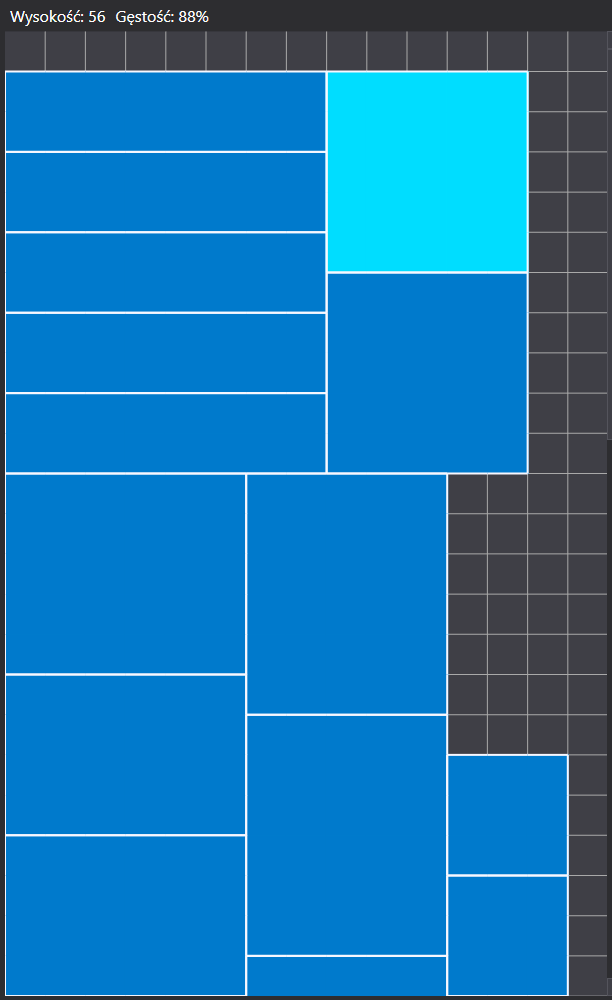
\includegraphics[width=0.7\textwidth]{prostokaty_dziury.PNG}
\caption{Górna część wyniku dla funkcji dziur}
\end{figure}


\item Funkcja minimalizująca wysokość

Gęstość dla $k=3$: 89

Najlepsza gęstość dla $k=4$: 91

Problemem w tej funkcji okazał się fakt, że na końcu nie zostały żadne wąskie klocki - wcześniej zostały wykorzystane, bo kładzenie ich poziomo pozwalało na chwilową minimalizację wysokości.
\begin{figure}[H]
\centering
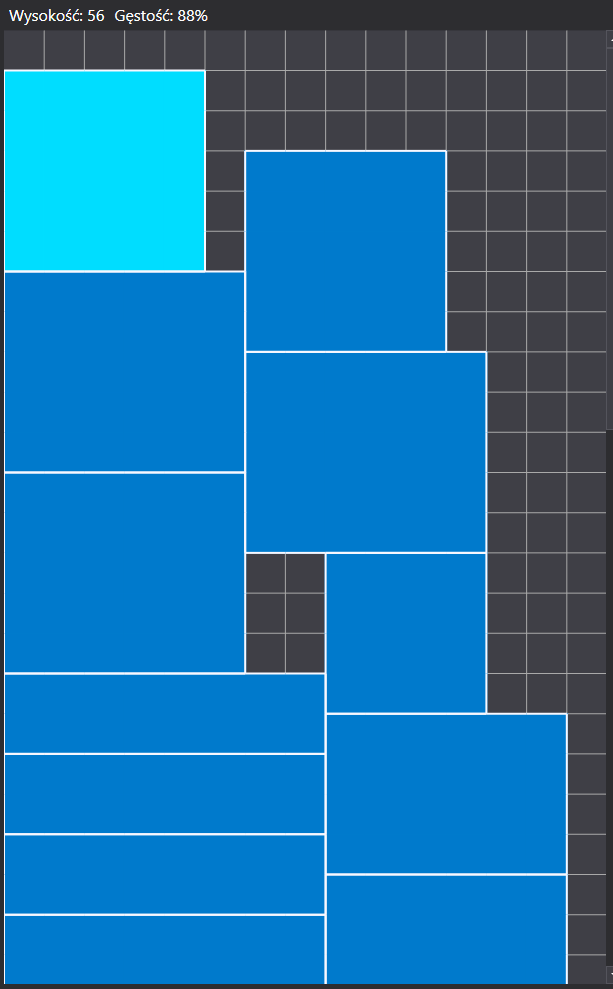
\includegraphics[width=0.75\textwidth]{prostokaty_wysokosc.PNG}
\caption{Górna część wyniku dla funkcji wysokości}
\end{figure}

\item Funkcja maksymalizująca przyleganie

Gęstość dla $k=3$: 91

Najlepsza gęstość dla $k=5$: 96

Rozwiązanie dla $k=5$ wydaje się być bardzo dobre - być może najlepsze, jakie można uzyskać dla tego zadania.
\begin{figure}[H]
\centering
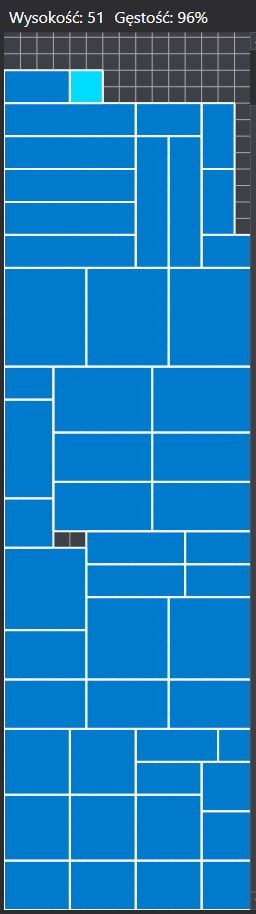
\includegraphics[width=0.35\textwidth]{prostokaty.PNG}
\caption{Najlepsze rozwiązanie dla prostokątów}
\end{figure}

\end{enumerate}
\subsection{Zestaw klocków o różnorodnych rozmiarach i kształtach (grupy Marcina Rudnika)}
Nasz algorytm dobrze radzi sobie z tym testem. 
Wynika to z kilku cech naszego rozwiązania.
Po pierwsze umożliwiamy wstawianie klocków w powstałe wcześniej dziury - na rysunku poniżej można zaobserwować kilka klocków, które idealnie gdzieś się wpasowały.
Ponadto funkcja przyległości (która okazała się najlepsza) faworyzuje duże klocki, co w tym wypadku jest korzystne - lepiej potem wypełnić powstałe dziury, niż najpierw szczelnie wypełnić dół planszy małymi klockami.
\begin{enumerate}

\item Funkcja minimalizująca dziury

Gęstość dla $k=3$: 73

Najlepsza gęstość dla $k=4$: 75

\item Funkcja minimalizująca wysokość

Gęstość dla $k=3$: 69

Najlepsza gęstość dla $k=69$: 73

\item Funkcja maksymalizująca przyleganie

Gęstość dla $k=3$: 78

Najlepsza gęstość dla $k=8$: 81

\begin{figure}[H]
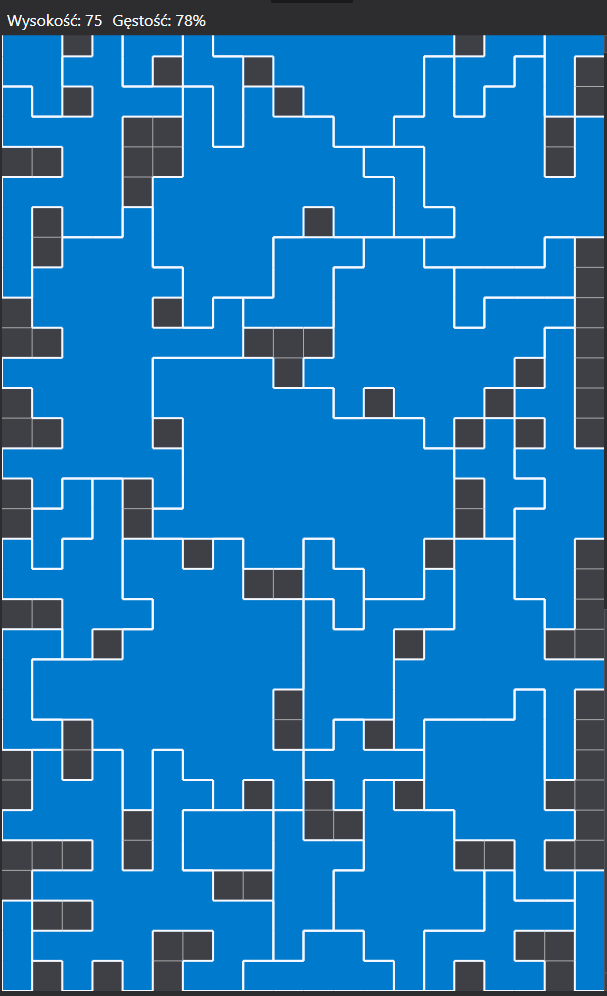
\includegraphics[width=\textwidth]{duze_klocki.PNG}
\caption{Ułożenie dużych klocków dla funkcji przyległości}
\end{figure}

\end{enumerate}


\subsection{Zestaw 120 klocków 5x4 o polu 9, z szerokością studni 10, grupy Mirona Marczuka}
\begin{enumerate}

\item Funkcja minimalizująca dziury

Gęstość dla $k=3$: 65

Najlepsza gęstość dla $k=7$: 68

\item Ulepszona funkcja minimalizująca dziury

Gęstość dla $k=3$: 73

Najlepsza gęstość dla $k=10$: 80

\item Funkcja minimalizująca wysokość

Gęstość dla $k=3$: 72

Najlepsza gęstość dla $k=8$: 78

\item Funkcja maksymalizująca przyleganie

Gęstość dla $k=3$: 68

Najlepsza gęstość dla $k=10$: 78

\end{enumerate}
\textbf{Wnioski}

W tym teście z wcześniej wykorzystywanych funkcji zdecydowanie odstawała jedynie funkcja minimalizująca dziury. Powód jest taki sam jak we wcześniej omawianym przykładzie -- algorytm pozostawia pustą kolumnę, co bardzo negatywnie wpływa na wynik. Z kolei wynik algorytmu minimalizującego wysokość jest bardzo dobry, bo wszystkie klocki mają bardzo zbliżoną wysokość i szerokość, tak więc algorytm nie próbuje po prostu położyć poziomo na spodzie wszystkich podłużnych klocków.

Testowo została wprowadzona tu omówiona wcześniej ulepszona wersja funkcji minimalizującej dziury, która okazała się w tym przypadku być najlepszą ze wszystkich, ponieważ usprawnienie rzeczywiście wyeliminowało tworzenie się pustej kolumny.

\subsection{Zestaw 124 klocków 5x4 i 6x4 o polu 9, z szerokością studni 80, grupy Anny Bekas}
Głównym problemem tego zestawu jest nieproporcjonalnie szeroka studnia w porównaniu do liczby i wielkości klocków.
\begin{enumerate}

\item Funkcja minimalizująca dziury

Gęstość dla $k=3$: 63

Najlepsza gęstość dla $k=5$: 66

\item Ulepszona funkcja minimalizująca dziury

Gęstość dla $k=3$: 66

Najlepsza gęstość dla $k=3$: 66

\item Funkcja minimalizująca wysokość

Gęstość dla $k=3$: 52

Najlepsza gęstość dla $k=4$: 66

Dla funkcji minimalizującej wysokość warto zwrócić uwagę na różnicę rozwiązań przy bardzo niewielkiej zmianie parametru $k$, a także fakt, że dalszy wzrost parametru $k$ nie miał już znaczenia.
\begin{figure}[H]
\centering
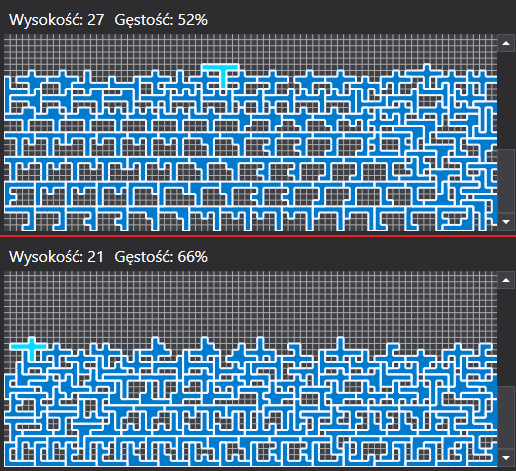
\includegraphics[width=\textwidth]{wysokosc_bekas.PNG}
\caption{Ułożenie klocków dla funkcji wysokości}
\end{figure}


\item Funkcja maksymalizująca przyleganie

Gęstość dla $k=3$: 63

Najlepsza gęstość dla $k=10$: 73

\end{enumerate}
\textbf{Wnioski}

Najlepsza okazała się funkcja maksymalizująca przyleganie. Dla funkcji minimalizującej dziury zwiększanie parametru $k$ nie poprawiało rezultatów, ze względu na bardzo szeroką studnię w stosunku do liczby klocków -- przez cały pierwszy wiersz w praktyce nie pojawiały się żadne dziury. Jej usprawniona wersja osiągnęła taki sam maksymalny wynik, ale dla trochę niższej wartości parametru $k$ -- tutaj powstawanie kolumny nie było znaczącym problemem.
Ciekawe zachowanie funkcji minimalizującej wysokość (duży przeskok z $k=3$ do $k=4$, a następnie brak poprawy) jest bardzo łatwy do wytłumaczenia -- zwiększenie $k$ ``zmusiło" algorytm do rozważenia znacznie lepszej rotacji, która na początku nie ma znaczenia, ale później decydowała o całym ułożeniu. 


\clearpage

\section{Podsumowanie testów} 
W testach prawie zawsze, nawet dla bardzo niestandardowych danych, najlepszą funkcją kosztu okazała się funkcja maksymalizująca przyleganie. Przy odpowiednio dużych, ale jednocześnie rozsądnych, wartościach parametru $k$ (nie większych niż 10) nawet dla najtrudniejszych przypadków gęstość nie spadała poniżej 70\%. Ceną za najwyższą skuteczność jest najdłuższy czas działania algorytmu w przypadku wyboru tej funkcji -- nie jest to jednak znaczący problem ze względu na ogólną wysoką wydajność algorytmu.

Funkcja minimalizująca wysokość zawsze zachowywała się w bardzo przewidywalny sposób -- kładąc wszystkie klocki poziomo, zaczynając od tych najbardziej podłużnych, co zwykle nie dawało optymalnego położenia. Często klocki były położone płaską stroną do góry, co znacznie pogarszało jakość rozwiązania, i dopiero po zwiększeniu wartości parametru $k$ rozważane były warianty z poprawnym obrotem. Rozwiązania funkcji minimalizującej wysokość były dobre głównie w sytuacji, gdy wszystkie klocki miały bardzo zbliżoną wysokość i szerokość (np. 5x4). Jej czas wykonania był szybki, ale porównywalny ze zwykle lepszą funkcją minimalizującą liczbę dziur.

Funkcja minimalizująca liczbę dziur często osiągała wyniki niewiele gorsze, a czasem nawet lepsze, niż funkcja maksymalizująca przyleganie. Jej główną wadą były tworzące się puste kolumny -- nie były uznawane za dziury. Jej ulepszona wersja, która jako dziury dodatkowo uznawała wszystkie puste pola poniżej średniego poziomu, rozwiązała ten problem i znacząco poprawiła jakość rozwiązania, które wcześniej było ograniczone tym mankamentem. Poprawka ta jednak nie wpływa na drugie ograniczenie tej funkcji -- bardzo szerokie plansze, na których dziury przez długi czas w ogóle nie występują, a jak zaczynają występować, jest już za późno, żeby to naprawić. Dużą zaletą tej funkcji była kilkukrotnie większa szybkość, niż funkcji maksymalizującej przyleganie, mimo dawania niewiele gorszych rezultatów.

Jednym z czynników, który wpływa na dobre wyniki algorytmu nawet dla granicznych przypadków, jest brak zależności od jakichkolwiek ukrytych stałych. W miejscach, w których można było rozważyć wykorzystanie ich (jak na przykład w ulepszonym wariancie funkcji minimalizującej liczbę dziur), wykorzystane zamiast tego były wartości zależące od rozwiązania (np. średnia wysokość kolumn w planszy). Dzięki temu również powinno być zachowane identyczne działanie algorytmu po przeskalowaniu planszy i klocków (na przykład dwukrotnym powiększeniu lub pomniejszeniu).

Wartym zauważenia jest fakt, że zwiększanie parametru $k$ nie zawsze poprawia jakość otrzymanego rozwiązania. W niektórych przypadkach od pewnego momentu jakość już nie wzrasta, a w niektórych nawet się pogarsza. Oczywiście dla odpowiednio dużego $k$ rozwiązanie musi być lepsze (bo dla odpowiednio dużej wartości $k$ sprawdzane jest każde rozwiązanie), ale dla ``rozsądnych" wartości (do 10) można zauważyć taki efekt, co, jak zostało wcześniej wyjaśnione, wynika z zachłannej natury algorytmu.




\end{document}